\documentclass[]{scrartcl}


\usepackage[english]{babel}
\usepackage{euscript}
\usepackage[utf8]{inputenc}
\usepackage[ruled,vlined]{algorithm2e}

\usepackage{graphics}

\usepackage[dvips]{graphicx}

\pagestyle{headings} \makeatletter

\usepackage{verbatim}


\usepackage{pictexwd,dcpic}


% quotient re-definition
\def\quotient#1#2{%
    \raise1ex\hbox{$#1$}\Big/\lower1ex\hbox{$#2$}%
}

% Margins
%\addtolength{\textwidth}{1cm}
%\addtolength{\marginparsep}{2cm}

\usepackage{makeidx}
\usepackage{eurosym}
\usepackage{amsfonts}
\usepackage{latexsym}
\usepackage{makeidx}
\usepackage{amsmath}
\usepackage{amsthm}
\usepackage{amscd}
\usepackage{comment}
\usepackage{enumerate}
\usepackage{mathrsfs}
\usepackage[all]{xy}

\DeclareMathOperator*{\argmax}{arg\,max}
\DeclareMathOperator*{\argmin}{arg\,min}

\usepackage{url}
\usepackage[colorlinks=true, a4paper=true, pdfstartview=FitV,
linkcolor=blue, citecolor=blue, urlcolor=blue]{hyperref}


\newtheorem{theorem}{Theorem}[section]
\newtheorem{corollary}{Corollary}[theorem]
\newtheorem{lemma}[theorem]{Lemma}

\theoremstyle{definition}
\newtheorem{definition}{Definition}[section]

%opening
\title{Bourbaki vs Pragmatism \\ A methodological comparison through the multi-armed bandits problem
 \\
 DRAFT
}
\author{Sebastiano Ferraris\footnote{sebastiano.ferraris@gmail.com}}

\begin{document}

\maketitle

% ------------------------------------------------- %
\begin{abstract}
    In these pages, through the example of the the multi-armed bandit problem, you will find a comparison between two methodological approaches to mathematics.
    The two methods are here named the \emph{Bourbachist} and \emph{pragmatic}: the Bourbachist way is concerned with the mathematical foundation upon which a formal solution emerges from a set-theoretical axiomatic structure. The other way, the pragmatic one, is focused on the algorithmic solution, and any underpinning mathematical formalisation appears only when needed.
    In this article you can also find a brief literature review about the history and origin of Bourbachism, and a shortlist of other notable examples where the same problem has been addressed in the Bourbachists' and in the pragmatic way. The article concludes with a final discussion about the advantages and disadvantages of each approach. \\

\noindent
If you discovered this article while searching for an introduction to the multi-armed bandit problem, please look directly at section~\ref{se:pragmatic_perspective}. The code to create the figures, to run and compare a range of solutions to the multi-armed bandit problem is version controlled and open to contributions at the link \href{https://github.com/SebastianoF/multi-armed-bandits-testbed}{https://github.com/SebastianoF/multi-armed-bandits-testbed}.
\end{abstract}


% ------------------------------------------------- %
\section{Two ways to approach the multi-armed bandits problem}
\label{se:intro}
Imagine you have to repeatedly choose between $K$ different options. All options have the same cost, though each may or may not provide you with a reward. The probability of having a reward is modelled by an \emph{unknown} distribution, that may be different for every option and that can vary over time.

This general setting is of concern for a wide range of problems, such as choosing a medical treatment or a drug, randomising quality control of produced parts, exploring new cafes, trying a range of cars before buying one, choosing a job, and for the most daring ones, selecting a partner. In the algorithmic literature the setting is referred to as the \emph{multi-armed bandits} (MAB), as it can be seen as the situation of playing repeatedly at a row of $K$ slot machines, and after the nickname \emph{armed bandit} for slot machines.

The reason why the algorithm takes its name form the gambling example and not from one of the others, more interesting and available in literature\footnote{
    For example Bouneffouf~\cite{bf2019survey}.
    }
is that the gambling case is the easiest to generalise and the one where the algorithmic machinery employed is also easier to visualise.
So, following the tradition, imagine to be on a trip to Las Vegas with an initial amount of money to invest in a row of $10$ slot machines. Let's say you start with $\$1000$, and that each draw costs $\$1$, this gives you $1000$ attempts to play and to balance an \emph{exploration} phase with an \emph{exploitation} phase. In the exploration phase the goal is to find an estimate for the unknown distributions of each arm. The exploitation phase aims at using the acquired knowledge to gain the highest possible reward in the face of uncertainty\footnote{
    Thompson~\cite{thompson1933likelihood} provides an early exposition to the method where the two arms are two medical treatments, Bellman~\cite{bellman1956problem} formulates the problem in a Bayesian perspective, again for two arms, and the more recent Sutton~\cite{sutton2018reinforcement}, Chapter~1, considers the problem as a starting point to introduce the field of reinforcement learning.
}.

The goal here is to provide a solution to the MAB problem, following two different mathematical approaches:
\begin{itemize}
    \item[$\circ$] \emph{Bourbachist approach.} Started in 1934 by a group of French mathematicians and named after a collective pseudonym, the Bourbachist school is driven by the need of providing a strict formalisation of the theory from a set theoretical perspective, so that all the conclusions are a consequence of a list of axioms, excluding any physical intuition.
    \item[$\circ$] \emph{Pragmatic approach.} In contrast to the Bourbachist approach, the pragmatic one reduces the formalisation to its bare minimum, and it orientates the reader's efforts into finding a solution of a problem usable in practice, rather than creating a rigorous axiomatic theory.
\end{itemize}

Historically, the original goal of the Bourbaki group was to re-write one of the most widely used analysis textbook of the time, the Goursat’s \emph{Cours d'analyse mathématique}, after a few counterexamples contradicting some statements were found (Marmier~\cite{marmier2014idea}). To this end the Bourbachists rewrote the standard analysis into an axiomatic system, detached from any physical intuition, and as rigorous as possible to avoid counterexamples. From this starting point they aimed at rewriting the whole corpus of mathematical analysis into a theory grounded on set theory and axiomatic systems. The feature that can be found in all books produced by Bourbaki, other than a set theoretical foundation, is that any connection with the physical reality as well as the history motivating the given theorems are entirely omitted from their textbooks.

In its opposition stands what is called here pragmatic approach. This is a solution oriented approach, where the concern towards rigorous definitions and foundations only relates to what is needed to solve the given problem. 

These categorisation of mathematics, an any categorisation, has some drawbacks. To better clarify we will use the MAB problem as an example. This will be formalised \emph{à la Bourbaki} in the next one, and subsequently in the pragmatic way in section~\ref{se:pragmatic_perspective}.

% ------------------------------------------------- %

\section{The Bourbachist way}
\label{se:bourbaki_perspective}

\begin{definition}
    Let $(\Omega, \mathcal{A})$ be a $\sigma$-algebra defined as a non-empty set $\Omega$ paired with a subset of its power set $\mathcal{A}$, containing the empty set, and closed under numerable union and complement set. Let this be called an \emph{action space}. Let $\mathcal{I}_{K} = \{1,2, \dots , K\} \subset \mathbb{N}$ be a set of indexes whose generic element $k$ is called an \emph{arm}, by convention. Let $\mathcal{I}_{T} = \{1,2, \dots , T\} \subset \mathbb{N}$ be another set whose elements are called, again conventionally, \emph{time}. Let $\mathbb{R}_{+}$ be the positive real axis including the zero.
\end{definition}

The relationship between the above defined elements are given by an invertible function function $A$, defined as:
\begin{align*}
    A : \mathcal{I}_T \times \Omega &\longrightarrow \mathcal{I}_K \\
        (t, \omega) &\longmapsto A(t, \omega) = A_t(\omega)
\end{align*}
and by a function $\mathcal{R}$, defined as:
\begin{align*}
\mathcal{R} : \mathcal{I}_T \times \Omega &\longrightarrow \mathbb{R}_{+} \\
(t, \omega) &\longmapsto \mathcal{R}(t, \omega) = \mathcal{R}_t(\omega)
\end{align*}
Let the former be called \emph{action} and the latter be called \emph{reward}. 
We add to $A$ the property of $A_t^{-1}(\omega) \in \mathcal{A}$, for each $t \in \mathcal{I}$.
Let
\begin{align*}
R : \mathcal{I}_T \times \mathcal{I}_K &\longrightarrow \mathbb{R}_{+} \\
(t, \omega) &\longmapsto R(t, k) = R_t(k)
\end{align*}
be another function, based on which the function $\mathcal{R}$ becomes the composition  that makes the diagram below commutative, for each $t \in \mathcal{I}$:

\[
\begindc{\commdiag}[20]

% --- nodes:

% below
\obj(0,30)[R]{$ \mathbb{R}_{+} $}

% above
\obj(0,60)[Ik]{$ \mathcal{I}_K $}
\obj(-40,60)[A]{$ \mathcal{A} $}

% --- arrrows

% ortho
\mor{Ik}{R}{$R_{t}$}
\mor{A}{Ik}{$A_t$}

%  oblique
\mor{A}{R}{$\mathcal{R}_t$}

\enddc
\]
%
Let $R_t$ be called the \emph{reward's realisation}, or simply $\emph{reward}$ when there is no ambiguity.\\
We observe that $\mathcal{R}$ maps the elements $\Omega$, while $R$ maps the corresponding indexes, as their realisations. 

Now we consider
\begin{align*}
    \mathcal{Q} : \mathcal{I}_T \times \mathcal{A} &\longrightarrow \mathbb{R}_{+} \\
        (t, \omega) &\longmapsto \mathcal{Q}(t, \omega) = \mathcal{Q}_t(\omega)
\end{align*}
and we call it the \emph{estimated reward of the action $\omega$ up to time $t$}, for $\omega = A_t^{-1}(k)$ for a fixed $k\in \mathcal{I}_K$, with the corresponding function $Q: \mathcal{I}_T \times \mathcal{I}_K \rightarrow \mathbb{R}$. It follows that $\mathcal{Q}$ is defined as an application of the mean value in a Lebesgue space over $(\Omega, \mathcal{A})$, that is now a Borel $\sigma$-algebra\footnote{
    For a foundational perspective, see Bourbaki~\cite{bourbaki2004integration}.
} as:

\begin{align}\label{def:mathcalQt}
\mathcal{Q}_t(\omega) = \mathbb{E} \left[ R_{\tau}(k)\mid k = A_{\tau}(\omega)~~ \forall \tau \in \mathcal{I}_t \right]
\qquad
\omega \in \mathcal{A}
\qquad
t \in \mathcal{I}_T
\end{align}
and therefore its realisation
\begin{align}\label{def:Qt}
Q_t(k) = \mathbb{E} \left[ \mathcal{R}_{\tau}(\omega)\mid \omega = A_{\tau}^{-1}(k)~~ \forall \tau \in \mathcal{I}_t \right]
\qquad
t \in \mathcal{I}_T
\qquad
k \in \mathcal{I}_K
\end{align}
As $\mathcal{R}$ and $R$ did, also $\mathcal{Q}$ and $Q$ satisfies the commutativity of a diagram analogous to the one shown above. The notation can be simplified for brevity to:
% \footnote{
%     The simplified notation is often the only notation appearing in engineering textbooks (e.g. Sutton~\cite{sutton2018reinforcement}), although this would not allow you to understand the subtle formalisation of assigning to an event $\omega$ its index $k$. More tragically, if only the simplified notation is introduced, some may call that the concepts introduced before irrelevant and pedantic.
% } to:
\begin{align}\label{def:mathcalQt_simple}
Q_t(k) = \mathbb{E} \left[ R_{t}(k) \mid A_{t} = k \right]
\end{align}
where the mean value is for all the time indexes up to $t$ and where the domain values of $A_t$ is clear from the context. We remind the reader that the $k$ is constant to be constant for each $t\in\mathcal{I}_t$. We are now writing a definition that will be of use when we will be extending $k$ to be varying over $t$.

\begin{definition}
    Let the \emph{total reward} $Q_{\infty}: \mathcal{I}_K \rightarrow \mathbb{R}$ be the function
    \begin{align}\label{def:mathcalQinf}
    Q_{\infty}(k) = \mathbb{E} \left[ \mathcal{Q}_{t}(\omega) \mid \omega = A^{-1}_{t}(k)~~ \forall t \in \mathcal{I}_T \right]
    \qquad
    k \in \mathcal{I}_K
    \end{align}
    or with the simplified notation as:
    \begin{align}\label{def:mathcalQinf_simple}
    Q_{\infty}(k) = \mathbb{E} \left[ R_{t}(k) \mid A_{t} = k \right]
    \end{align}
\end{definition}

So far we have been considering the reward and the total reward for a fixed choice of $k$. We can vary $k\in \mathcal{I}_K$ in function of the time index. So let $\mathbf{k}$ be an element of
\begin{align*}
\mathcal{I}_K^T = \underbrace{\mathcal{I}_K\times \mathcal{I}_K \times \dots \times \mathcal{I}_K}_{T\text{-times}}
\end{align*}
or equivalently a function from $\mathcal{I}_T$ to $\mathcal{I}_K$.
Definitions \ref{def:mathcalQt} and \ref{def:mathcalQt_simple} are so generalised to $Q_t:\mathcal{I}_K^T \rightarrow \mathbb{R}$ for $t\in\mathcal{I}_{\leq T}$, having defined $\mathcal{I}_{\leq T}$ any interval of positive integers between~$1$ and $T$, and
\begin{align*}
Q_t(\mathbf{k}) = \mathbb{E} \left[ \mathcal{R}_{\tau}(\omega)
\mid
\omega = A^{-1}_{\tau}(\mathbf{k}_{\tau})~~ \forall \tau \in \mathcal{I}_t \right]
\qquad
\mathbf{k} \in \mathcal{I}_K^T
\qquad
t \in \mathcal{I}_T
\end{align*}
and therefore
\begin{align*}
Q_{\infty}(\mathbf{k}) = \mathbb{E} \left[ \mathcal{R}_{t}(\omega)
\mid
\omega = A^{-1}_{t}(\mathbf{k}_{t})~~ \forall t \in \mathcal{I}_T \right]
\qquad
\mathbf{k} \in \mathcal{I}_K^T
\end{align*}
The mean value computed with a Lebesgue measure, over the Borel space generated as the sets of images\footnote{
    We consider the definition under the accordance with the axiom of choice as in the ZFC axiomatic set theory, in order to avoid \emph{virages dangereux}. See also Bourbaki~\cite{bourbaki2004theory} and \cite{takeuti1982classes}.
} $\mathcal{R}_t(\omega)$ for all $\omega \in \mathcal{A}$ can be reformulated as:
\begin{align*}
Q_t(\mathbf{k})
=
\frac
{\sum_{\tau=1}^{t} R_{\tau}(\mathbf{k}_{\tau}) \mathbf{1}_{A_\tau = \mathbf{k}_{\tau}}}
{\sum_{\tau=1}^{t} \mathbf{1}_{A_\tau = \mathbf{k}_{\tau}}}
\end{align*}
where $\mathbf{1}_{A_\tau = \mathbf{k}_{\tau}}$ equals to $1$ for when the event $\omega$ corresponding to $\mathbf{k}_{\tau}$ is mapped exactly to $\mathbf{k}_{\tau}$ through $A_t$, and $0$ for any other event.
Extending the time indexes up to infinity, and to justify the notations introduced above, where we used $\infty$ for the finite case, we have the following theorem:
\begin{theorem}\label{th:bourbaki}
Given a ring of infinite cardinality to which the time index $t$ belongs, and an Hilbert module\footnote{An algebraic structure generalising Hilbert vector spaces over the now introduced ring of time indexes. See for example \cite{bourbaki1987topological}.} to which the vector $\mathbf{k}$ belongs, it follows that
\begin{align*}
Q_{\infty}(\mathbf{k}) = \lim_{T \rightarrow \infty} Q_{T}(\mathbf{k})
\end{align*}
\end{theorem}
\begin{proof}
    Direct consequence of the definition of $Q_{\infty}$. Details left to the reader.
\end{proof}

We now consider the value $\hat{k}$ that satisfies
\begin{align*}
\hat{k} = \argmax_{k \in \mathcal{I}_K} Q_t(k)
\qquad
\forall t \in \mathcal{I}_T
\end{align*}
for a constant value for each time index, as in the definition~\ref{def:Qt} of $Q_t$.
If you consider the possibility of varying the chosen arm $k$ across time, and so if you are allowed to compare different images of the function $A_t$, then $\hat{\mathbf{k}}$ is defined as
\begin{align}\label{eq:bourbaki_solution}
\hat{\mathbf{k}}
=
\argmax_{\mathbf{k} \in \mathcal{I}_K^{T}} Q_t(\mathbf{k})
\qquad
\forall t \in \mathcal{I}_T
\end{align}
Under the light of theorem~\ref{th:bourbaki}, and with the given definitions, we can now call the so defined vector $\hat{\mathbf{k}}$ the \emph{solution of the generalised multi-armed bandits problem}.

The attentive reader may have noticed a caveat. The realisation $R_t$ appearing in the first diagram, is defined upon a stochastic process, but it does not have the property of being random, in the sense that it is not define upon a sigma algebra. This abuse of notation to allow for a realisation is not the only possible option to re-build the whole axiomatic system.

To avoid this impasse that may cause contradictions in future developments based on the axiomatic structure given so far, we can instead define $R_t$ as the stochastic process:
\begin{align*}
    R_t : \Omega \times \mathcal{I}_K &\longrightarrow \mathbb{R}_{+} \\
    (\omega, k) &\longmapsto R_t(\omega, k)
\end{align*}

Now we define $\tilde{A}_t$ as the inverse of the projection of the first set $\pi_1 : \Omega \times \mathcal{I}_k \rightarrow \Omega$, $\tilde{A}_t = \pi_1^{-1}$, and $\mathcal{R}_t$
as the composition:

\[
\begindc{\commdiag}[20]

% --- nodes:

% above
\obj(-40,60)[Omega]{$ \Omega $}

% below
\obj(-40,30)[OmegaI]{$ \Omega \times \mathcal{I}_K $}
\obj(0,30)[R]{$ \mathbb{R}_{+} $}



% --- arrrows

% ortho
\mor{Omega}{OmegaI}{$\tilde{A}_t$}
\mor{OmegaI}{R}{$R_t$}

%  oblique
\mor{Omega}{R}{$\mathcal{R}_t$}

\enddc
\]
%

\noindent
As an exercise, the reader can reformulate the theorem~\ref{th:bourbaki} starting from the new definition of $R_t$ given above.


% ------------------------------------------------- %
\section{The Pragmatic way}
\label{se:pragmatic_perspective}

The first step to approach the problem pragmatically is to implement a playground where the ground truth of an instance of a multi-armed bandit problem is known. 

\subsection*{Creating a Benchmark}

We first implement a particular case, modelling each arm with normal distributions, with mean sampled from a uniform distribution in the interval $[-3, 3]$ and the standard deviation sampled from a uniform distribution on the interval $[2, 3]$. A representation of these distribution is plotted in
figure~\ref{fig:volin_plot}.

If the studied case is modelled with a different distribution, what is said in this section is still applicable by simply adapting this benchmark to the intended situation.

\begin{figure}[h]
    \hspace{-1.5cm}
    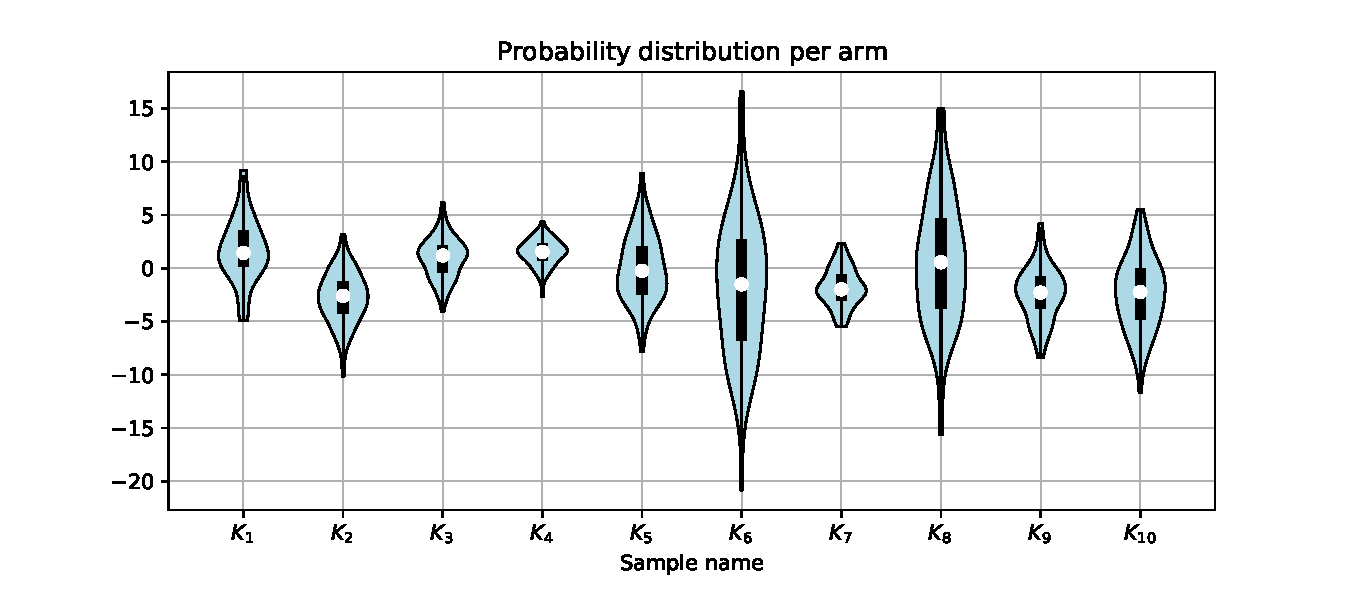
\includegraphics[width=18cm]{figures/initial_distributions.pdf}
    \caption{The distributions of the random reward for each arm $K$, unknown to the player, are sampled from normal distributions, with mean uniformly sampled in the interval $[-3, 3]$ and standard deviation in the interval $[1, 2]$.}
    \label{fig:volin_plot}
\end{figure}

\subsection*{Encoding the problem}
The player gains a reward after pulling an arm index $k$, for each time point $t$. We encode the rewards in a $T\times K$ \emph{reward matrix} $q$. In our example $T=1000$ is the largest time we will be pulling an arm and $K=10$ is the number of arms. The element $q_{t, k}$ represents the reward collected for having pulled the arm $k$ at the time-point $t$. As we can pull only one arm at a time, there is only one known value for each row of the matrix. All the other values are initialised to nan.

The multi-armed bandit is defined by two vectors $\mu$ and $\sigma$, where $\mu_k$ is the mean and $\sigma_k$ is the standard deviation of the distribution of the arm $k$.
To consider the non-stationary case, where the means and the standard deviations of the arms' distributions represented in Figure~\ref{fig:volin_plot} are not constant over time, we turns the vector $\mu$ and $\sigma$ into matrices of size $T_{\text{arm}} \times K$, providing the mean and standard deviation of the distribution of the arm $k$ at time $t$.

The rewards can be accumulated for greater or fewer time points than $T_{\text{arm}}$, as the distributions of the arms can repeat. If $T_{\text{arm}}=1$ then the problem is stationary, and if $T=30$ and $T_{\text{arm}}=15$ then each arm $k$ will be looping over its parameters $\mu_{:, k}$ and $\sigma_{:, k}$ twice, according to:
\begin{align*}
q_{t, k}
=
\text{norm}\left(\mu({t~\text{mod}~T_{\text{arm}}, k}), \sigma({t~\text{mod}~T_{\text{arm}}, k})\right)
\end{align*}
where $\text{norm}(\mu, \sigma)$ is the normal distribution of location $\mu$ and scale $\sigma$ and mod is the modulo operator.

\subsection*{$\epsilon$-greedy algorithms}

In the previous section we created a benchmark and encoded the multi armed bandit response/rewards into a matrix.

\begin{figure}[h]
    \hspace{-1cm}
    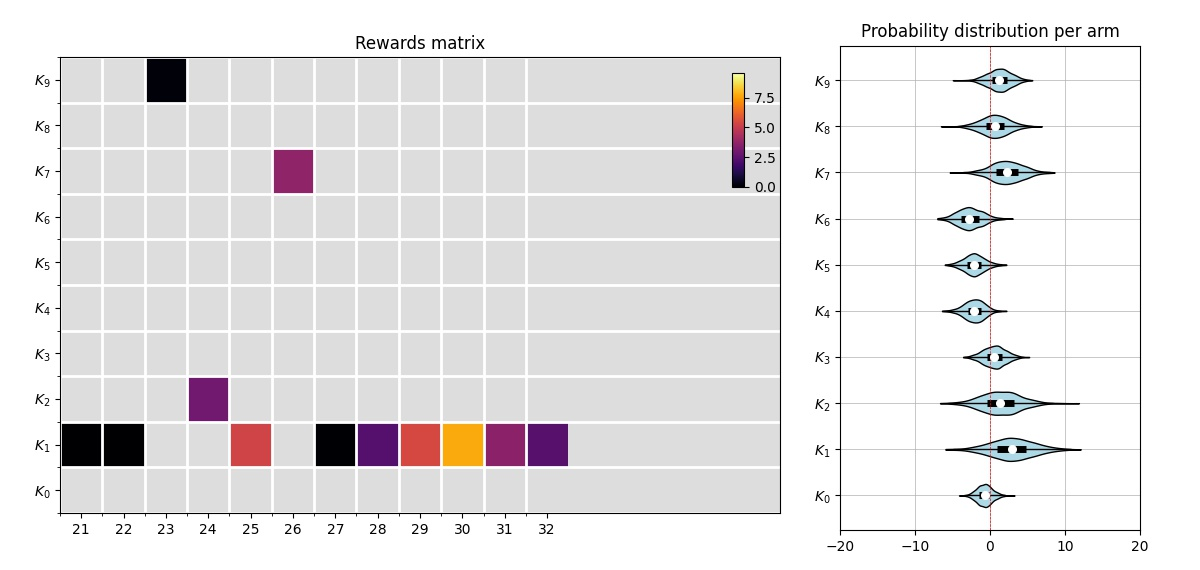
\includegraphics[width=17cm]{figures/step_32.jpg}
    \caption{The reward matrix after $32$ steps of a \emph{naive} $\epsilon$-greedy algorithm. We can see that step $23$, $24$ and $26$ are explorations in a row of exploitation of the arm $7$ that so far had produced the highest reward. To the grey colour corresponds the nan value used to initialise the reward matrix. In this instance, the reward is clipped at zero, as the loss of money is only the cost of pulling an arm at each time-point.}
    \label{fig:step_32}
\end{figure}

Now we introduce the $\epsilon$-greedy algorithms,
a class of algorithms based on the idea that if your bad luck is consistent, probably it is not just bad luck. The player using these algorithms alternates between a phase of exploration (proportional to $\epsilon$ times), and a phase of exploitation (proportional to $1 - \epsilon$). In the first phase, the player acquires information about the structure of the problem regardless the immediate gain, and in the second one, the information gained are exploited to maximize the . An historical introduction can be found in Chapter~1 of~\cite{sutton2018reinforcement}.

The basic version of the $\epsilon$-greedy algorithm (or \emph{naive $\epsilon$-greedy}), selects a random arm when exploring, and selects the best arm when exploiting. The algorithm can start with an initial phase of pure exploration, where only random arms are pulled. Figure~\ref{fig:step_32} shows this case.

A more sophisticated version the naive $\epsilon$-greedy is the \emph{best reward $\epsilon$-greedy}. Here, instead of selecting any random arm in the exploration phase, we weight the random selection using the rewards obtained so far, excluding the arm with the highest reward. With this strategy we will be more likely to explore the arms that have provided good rewards in the past, and to refrain from spending money over an arm that have never provided any gain at all.

A third algorithm is the \emph{least explored $\epsilon$-greedy}. In the exploratory phase of this algorithm we increase the probability of falling over the least explored arms, instead of the one providing the highest reward. This method and the previous one are both aimed at preventing from getting stuck in a local minimum, i.e. believing that the arm we are hitting is the best one, as it happens to provide a gain, though it is not the one with the optimal gain.

The fourth algorithm here presented is the \emph{upper confidence bound $\epsilon$-greedy algorithm} \cite{sutton2018reinforcement}. In this algorithm the estimated optimal arm at time $t$, is given by
\begin{align}\label{eq:upper_confidence_formula}
\hat{k}_t = \argmax_{k} \left[ \hat{\mu}(k) + \lambda \sqrt{ \frac{\ln(t)}{ N_{t}(k) }  } ~\right]
\end{align}
where $N_{t}(k)$ is the number of times the armed $k$ had been pulled up to the time $t$, which can be easily computed from $q$. The regularisation term weights the uncertainty in the estimate, correcting for possible underestimations of the mean.

Note that in this version of the game, the player will receive $0$ when the sampled reward is below $0$. This means that the estimated mean does not correspond to the one of the original distribution, though the result will be conservative in having an observed average close to zero for distribution whose mean is below the zero. You should resist the temptation of estimating the arm using the mode instead of the average in equation~\ref{eq:upper_confidence_formula}. In fact if the standard deviations are very different across arms, a very inconvenient arm, with the average below the zero, may be identified as the optimal one.

The performance of these algorithms are all depending upon the problem's distributions, and the optimal one should be found empirically via simulation. Providing a benchmarking for a general case would not be useful here. What provides the constraints to make the case less general, is based on the instance of the problem to which the algorithms are applied. A platform where to make further experiments is open-sourced and can be found at~\href{https://github.com/SebastianoF/multi-armed-bandits-testbed}{https://github.com/SebastianoF/multi-armed-bandits-testbed}.


% ------------------------------------------------- %
\section{Comparison}
\label{se:outro}

The Bourbaki way presented in section~\ref{se:bourbaki_perspective} is based on an axiomatisation of the problem and it evolves from a functional and set-theoretical perspective. It focuses on the symbolism, and according to the Bourbachist tradition, it provides no examples or algorithms, as the only connecting point between the theory and the given problem is the axiomatic setting.

Assuming that section~\ref{se:bourbaki_perspective} is correct (excluding typos) and coherent (excluding Goedel\footnote{
    In the critical article \emph{The ignorance of Bourbaki}~\cite{mathias1992ignorance} Mathias noticed that the Bourbaki attempt of grounding the whole corpus of mathematics in an axiomatic sense have happened after, and with a conscious effort to ignore the Goedel incompleteness theorems.
}), it is easy to see that the Bourbaki approach, while describing a rigorous and formal setting, wraps a relatively simple problem into several layers of complexity.
The pragmatic approach of section~\ref{se:pragmatic_perspective} shows instead that there is no need to take a functional perspective, when a single matrix is enough. Borel spaces and Lebsgue Measures are never mentioned, as these tools have been developed in entirely different contexts. Also the pragmatic approach reduces the bibliography to one or two resources.

\subsection*{Other examples}

If the MAB problem is considered too empirical to be a good case study for the proposed comparison, it is good to remind that the Bourbaki group intended to formalise the whole corpus of mathematics. In fact there are in the literature numerous examples where the Bourbachisation took place. 

The first and most notable one belongs to the domain of optimal transport theory. Started as a pragmatic tool of solve a class of optimisation problems, it had been turned, after the Bourbachists formalisation, into a $500$ page book underpinned by a large amount of measure theory and Lebesgue spaces, whose relevance to solve any instance of an optimal transport problem is debatable. It is possible to compare Hitchcock's~\cite{hitchcock1941distribution} introduction to its formalised counterpart, written by Villani~\cite{villani2003topics}: the first work is can be read in one sitting, and the material provided is enough to start implementing and possibly extending a solution to the optimal transport problem, with no more knowledge than the one provided in the high school. The second one, whose aim is the rigorous formalisation of what is needed to solve the problem, requires many years of academic studies only to grasp the first few pages. Here again the advantages in finding a numerical solution to the problem is debatable.

The second Bourbachisation example is in the domain of medical image registration. The aim of this field is to solve the problem of finding the non-rigid deformation, or metamorphosis, between anatomies. The problem originates from the study of the growth and change of anatomical shapes by D'Arcy Thompson~\cite{d1942growth} and pragmatically extended, amongst others, by Modersitzki~\cite{modersitzki2004numerical}. The Bourbaki rigorous version can be found in works such as Younes~\cite{younes2010shapes}, where the reason motivating the work can be found only at chapter 12.
In this case too, the advantages of the axiomatic approach are in respect to the pragmatic one, which appeared half a century earlier, are debatable.

For this specific case, the reader may say that the pragmatic approach \cite{modersitzki2004numerical} does not use neither diffeomorphisms nor reproducing Kernel Hilbert spaces. To this objection goes with the fact that it is not proved that neither diffeomorphisms nor reproducing Kernel Hilbert spaces are resulting in anything more accurate than their pragmatic counterparts when implemented in practice. Instead it is true that they are computationally slower and that they increase the cognitive load.


\subsection*{The Bourbaki pattern}

There are many other examples in the literature where it is possible to find a comparison between the Bourbachist / pragmatic way, such as with algebraic topology, fuzzy logic and topological data analysis. 
These branches of mathematics have been drawn out by Bourbachists from the practical set of solutions they were, into rigorous axiomatic constructions. As for the MAB problem, approaching the problem starting from these resource makes it very difficult to find any help in practically solving the given problem.

It is at this point evident the existence of a pattern in the process of Bourbachisation: a problem solved by more than 50 years, and often in a very elegant and straightforward way, is taken under the wing of the academic axiomatisers and transformed into a list of definitions, lemmas, theorems and corollaries, where no trace of the original problem motivating the theory is to be found. The pragmatic solution is reverse-engineered into a formal structure.

The formalised result is then called \emph{pure}, as opposed to \emph{applied}, leaving to intend the existence of a Platonic world of perfect and immutable ideas, whose applications are just sporadic instances. To allow to forget the fact that the applied mathematics was the source and origin of the axiomatic theory, the work of Bourbaki makes no reference to the history of the problem and the practical need that motivates each definition.

% The intriguing fact is that in the domain of philosophy, a similar pattern was deplored by Friedrich Nietzsche. Several decades before the advent of Bourbakism, in \emph{The Twilight of the Idols} the philosopher wrote: 

% \begin{quote}
%   \emph{
%       You ask me what all idiosyncrasy is in philosophers? [...] All the ideas that philosophers have treated for thousands of years, have been mummied concepts; nothing real has ever come out of their hands alive. These idolaters of concepts merely kill and stuff things when they worship,—they threaten the life of everything they adore.
%   }  
% \end{quote}

In the next section we dive into the pros and cons of the Bourbakist and the pragmatic approach, with some empirical considerations.

% -------------------------
% -------------------------
\section{Benefits and Drawbacks}


Despite many have express their negative view about the Bourbaki's work, the Bourbachist's mathematics is still widespread if not predominant across the academic community, as well as widespreadly taught.
Also very often, the over-axiomatisation of a solution to a practical problem developed outside academia, had received more recognition than the original work.

This section investigates the benefits and drawback of the two approaches, starting ffrom the pros of the Bourbaki methodology.

% -------------------------
\subsection*{Bourbaki benefits}

\begin{itemize}

    \item[$\circ$] \emph{Keeping counterexamples at bay:} this is the core reason why the group Bourbaki have started producing their work. The endeavour of avoiding counterexamples, even if possibly vain as pointed out by \cite{mathias1992ignorance}, can provide a range of abstract tools to probe the limits of a solution.
     
    \item[$\circ$] \emph{Exercise of rigour:} the Bourbaki approach is a valuable exercise of rigour and a way to master the mathematical formalisms. 
    
    \item[$\circ$] \emph{Uniformed language:} few mathematicians had a stronger impact in standardising and unifying notations across mathematical communities.

    \item[$\circ$] \emph{More publications:} the pressure of publishing is increasing as much as the difficulty in discovering new theorems and models. Formalising known theories is a way of producing papers\footnote{
        Same goes for publishing a comparisons between a range of mathematical approaches. This topic will be developed in another paper.
    }. Section~\ref{se:bourbaki_perspective}, once extended under the title \emph{The multi-armed bandits for the working mathematician} would provide a good candidate for a submission even if not containing any new result.
    
    \item[$\circ$] \emph{Detachment from reality:} the advantage of this point is twofold. Firstly, the Bourbaki approach entails no costs in running experiments or collecting data. Secondly, there is no objective measurement to score the quality or value of the Bourbaki work. Needless to say, this second point is an advantage only in the academic domain.
    
    \item[$\circ$] \emph{Good for the ego:} as all virtuosic expressions, also writing axiomatic structure is an exercise that, once mastered can lead to personal satisfactions, regardless of any practical value.
    
    \item[$\circ$] \emph{Inaccessible to novices:} also this point favours the Bourbaki way only in the academic domain. The jargon and the formalism that leaves everyone how is part of the Bourbaki club as an outsider is a possible strategy to maintain academic hierarchies intact.
    
    \item[$\circ$] \emph{Immune to failure or obsolescence:} addressing no practical problem, a theory developed following an axiomatic structure, or the axiomatisation of an existing solution, can not provide inherently \emph{wrong} results, and the axiomatisation can not become obsolete by emerging technologies, as it happens for the mathematics that solves practical problems.
    
    \item[$\circ$] \emph{(Almost) unconstrained research:} when the goal is to find all the possible results starting from a set of axioms, then the only constraints are the direction the mathematician chose to take, and the acceptance of the results from the other mathematicians in the same field.
     
\end{itemize}

% -------------------------
\subsection*{Bourbaki drawbacks}

Many mathematicians have express their negative view about the Bourbachist's mathematics, despite it being widespread if not predominant across the academic community. The most notable ones, other than the already cited Mathias \cite{mathias1992ignorance}, are Arnold~\cite{arnol1998teaching}, De Finetti~\cite{de2008bruno}, Lockhart~\cite{lockhart2009mathematician}, Velupillai~\cite{velupillai2012bourbaki}. Even a publication in favour of the Bourbaki style such as Marmier~\cite{marmier2014idea}, casts some shadow with its conclusions: \lq\lq Living mathematics is being done elsewhere in the world, in connection with new problems arising from other disciplines or other human activities\rq\rq.


\begin{itemize}

    \item[$\circ$] \emph{No new results:} unless considering the axiomatisation of a theory as a result \emph{per se}, it was very difficult to find breakthroughs or new results from the Bourbaki approach. The only notable exception to this point seems to be the work by Mochizuki~\cite{mochizuki2012inter}. This resource is claimed to have solved the \emph{abc conjecture}. Although, as reported by Castelvecchi~\cite{castelvecchi2015biggest} \emph{the proof is too impenetrable to be understood}.
     
    \item[$\circ$] \emph{Pedagogical failure:} a barbed letter by Vladimir Arnold~\cite{arnol1998teaching} denounce the failure of the Bourbaki methodology, in particular in its intention of separating physics from mathematics. He wrote: \lq\lq Mentally challenged zealots of \emph{abstract mathematics} threw all the geometry (through which connection with physics and reality most often takes place in mathematics) out of teaching.\rq\rq
    
    \item[$\circ$] \emph{More noise:} once formalised into axioms and theorems, it is a very arduous task to deduct the solution to the problem that motivated the axioms. A reader with no abstract mathematics background looking for a practical way to approach the multi armed bandit problem, would be drawn away from the problem by section~\ref{se:bourbaki_perspective}, if not entirely from mathematics. 
     
    \item[$\circ$] \emph{Less generalizable:} while this may seems not true at first glance, the reader is invited to continue the formalisation started in section~\ref{se:bourbaki_perspective}, to see how many pages and new definitions and diagrams are needed to formalise the case of arms whose distribution varies over time. Any small change in the original problem, that is of immediate intuition when the physical problem is at hand, requires days of work to keep the axiomatic system standing. Borrowing an example from \cite{arnol1998teaching}, proving the commutativity of the product is obvious when arranging soldiers in rows, long and tedious when axiomatising multiplication by the column method.
    
    \item[$\circ$] \emph{Hindrance of creativity:} Bruno de Finetti, playing on the Italian words \emph{assiomi} and \emph{matti} (crazy) coined the therm \emph{assiomatti}, to describe the mathematicians concerned with axiomatisation rather than solving problems or finding algorithms. The fact that formal structures comes into the way of the imagination and creativity was one of his thesis in criticising the Bourbaki method~\cite{de2008bruno}.

    \item[$\circ$] \emph{No layman way:} the only known attempt of turning a Bourbachist work into something accessible for the layman, can be found in Villani~\cite{villani2003livingtheorem}. The result admittedly makes the theory even less accessible than the original work.
    
    \item[$\circ$] \emph{Excessive rigour can be misleading:} besides the information overload cause by there Bourbaki approach, the detachment from practical problems can lead to blunders. An example of this can be found in the medical imaging paper by Lorenzi~\cite{lorenzi2013geodesics} where a counterexample found in Milnor~\cite{milnor1984remarks}, involving the tangent space of the circle, is used to justify the claims that there is no bijective correspondence between the space of the tangent vector fields and the one of their integral curves in $\mathbb{R}^3$, even if in plain contradiction with the theorem of existence and uniqueness of ODEs solutions.

    \item[$\circ$] \emph{Pure vs. Applied dichotomy:} the academic dichotomy pure/applied maths is something that can not be found in mathematics before Bourbaki. 
    Classifying any of the work by Archimedes, Gauss, Euler, Lambert, Poincare or any other great name of pre-modern mathematics as \emph{pure} or \emph{applied} with no ambiguities is an impossible task.
     
\end{itemize}

About this last point, several French mathematicians contemporary of Bourbaki, such as Jean Leray, René Thom, Paul Dubreil, and Szolem Mandelbrojt, have been labelled as \emph{applied} or \emph{not-pure}, for having left the Bourbaki group very early or for not having entered its ranks at all \cite{barcellos1984interview, atiyah2007bourbaki}.

It is possible to have the sensation that the pragmatics or applied mathematicians have found themselves with less and less space within the university walls after the emergence of the \emph{pure ones}. Having turned mathematics into something that is not practiced as a science, the members of the Bourbakist club endured and flourished in the academic positions, influencing how mathematics is taught, learned and conceived.

Of a similar idea were De Finetti~\cite{de2008bruno} and Arnold. The latter wrote:

\begin{quotation}
    \emph{Genuine mathematicians do not gang up, but the weak need gangs in order to survive. They can unite on various grounds (it could be super-abstractness, anti-Semitism or \lq\lq applied and industrial\rq\rq~problems), but the essence is always a solution of the social problem - survival in conditions of more literate surroundings.}~\cite{arnol1998teaching}
\end{quotation}

\subsection*{Pragmatic benefits}

\begin{itemize}
    \item[$\circ$] \emph{Practical value:} sometimes scientists browse mathematical papers to find an algorithm or a solution to one of the problems they are facing. The solution or algorithm is never to be found in the Bourbaki orientated publications.
    
    \item[$\circ$] \emph{Unbiased assessment:} it is possible to assess the quality of a mathematical theory with an objective measurement only if it solves a class or practical problem.
     
    \item[$\circ$] \emph{Constraints in doing research:} this is a consequence of the pragmatic mathematics being part of the scientific landscape. Research in the pragmatic mathematics is done through seeking solutions to problems, with constraints coming from its reality. This helps in not getting lost in a maze without a center, as it happens when only building mathematical structures upon set of axioms, as in the \emph{pure} counterpart.
      
\end{itemize}


\subsection*{Pragmatic Drawbacks}



\begin{itemize}
    \item[$\circ$] \emph{Lack of rigour:} a too strict definition of a basic concept can blind the intuition of the objet defined, although a non rigorous definition can make the consequent chain of deduction more difficult, if not impossible to attain.
    
    \item[$\circ$] \emph{Not for the ego-driven mathematicians:} it can be very frustrating to spend several months or years developing an algorithm or a solution, only to see it outpaced few years later (or few years back) by another mathematician. 
    The same does not happen in the Bourbaki approach.

\end{itemize}

About this last point, it was again Arnold who observed the concomitance of Bourbakism and inferiority complexes:

\begin{quotation}
    \emph{The ugly building, built by undereducated mathematicians who were exhausted by their inferiority complex and who were unable to make themselves familiar with physics, reminds one of the rigorous axiomatic theory of odd numbers. Obviously, it is possible to create such a theory and make pupils admire the perfection and internal consistency of the resulting structure 
    .}~\cite{arnol1998teaching}
\end{quotation}




% ------------------------------------------------- %
\section{In conclusion}

In this paper we used the multi-armed bandit problem as an example to compare the pragmatic and the Bourbakist approach to mathematics. From this starting point we provided a list of examples where the two methods have been used in literature to tackle the same problem, and we provided a consequent list of strengths and limitations of each approach. 

Compared to the history of mathematics, the Bourbachism is a relatively new trend, whose emergence required to separate between \emph{pure} and \emph{applied} mathematics. The Bourbaki group satisfied the need for unifying the language and the notation of mathematics in a more connected world, to detach mathematics as much as possible from physical reality, it provided a place where to exercise ones ability in manipulating abstract concepts and in turning intuitions into a rigorous formal language.

Although the overformalisation of ideas, and the shift of mathematics from being a tool to solve practical problems into the endeavour of building axiomatic structures, reshaped mathematics to be a mere intellectual exercise with several negative consequences. The methodological shift, paired with having called the intellectual exercise as the \emph{pure} one, leaving to intend the existence of a Platonic world of perfect axiomatic structures, mostly useless to anyone expecting help in solving practical problems. 

The preference between the two approaches is up to the reader, according to their needs, style and background. Nonetheless we reiterate the observation that the Bourbakist approach exists only within the walls of academia. Outside of it, mathematics is not a profession, as it is medicine or engineering, unless practiced in the pragmatic way.


\begin{small}
    \section*{Acknowledgements}

    Thanks to Jack Buckingham for reviewing the drafts of this paper and for the fruitful discussions. The author is the sole responsible for the content of the paper.
        
\end{small}



%Despite the fact that I am convinced that the students of the generations to come will be obliged to learn the Bourbaki sophistications to get a degree in mathematics, and to unlearn them as quickly as possible to be of any use to the non-academic society, I intended to show, alongside with many others before me (Mathias~\cite{mathias1992ignorance}, DeFinetti~\cite{de2008bruno}, Velupillai~\cite{velupillai2012bourbaki}, Arnold~\cite{arnol1998teaching}), that the Bourbaki method is around for academic reasons, and it is not what mathematics is about. % which is the application of the scientific method to understand the reality and to find the best algorithm that solves a given problem.

% Where the Bourbachism had shifted the focus from the problem to the axioms, and where you can only find an over-formalised list of definitions and theorems of no use outside academic discussions.

% When the pragmatic perspective is applied to the same problem, an algorithmic solution can be quickly explained, and the explanation is enough to provide the guideline to implement and test a range of algorithms. All this without calling into play Borel or Lebesgue, as done in the counterpart.



% If I wanted to divide the mathematical approaches into two, rather than Bourbaki and pragmatic, I would consider the Pythagorean and the Archimedean schools of thought. The Pythagorean school, started under the influence of the ancient Egyptian and Persian mathematicians, considers the mathematical practice as a tool to investigate and measure the reality and to find the connections between apparently distinct elements through abstraction and generalisation\footnote{
%     As for example astronomy, music and architecture~\cite{robins1995mathematics}, \cite{boyer2011history}.
% }, starting from the investigation of the concept of number itself.
% The Archimedean vision sees mathematics as a tool to solve very practical problems, approaching them with heuristic, algorithms and even adhoceries\footnote{
%     An example of this approach is the proof of the formula for the parabolic segment's area by Archimede~\cite{boyer2011history} and \cite{strogatz2019infinite}.
% }. To neither the Pythagorean nor the Archimedean belongs the dichotomy between pure and applied mathematics, as there is no concept of \emph{pure} in the sense of detached from the reality, being the reality always the centre of the investigation.






%
%
% in achieving a possible solution of a problem, and how choosing the wrong approach, would end up in never reaching anything useful. The paper shows the over-formalised approach first, and the pragmatic approach in the subsequent section.
%
%
%In the discussion we challenged the usefulness of the Bourbaki approach outside its circle of academics. The Bourbaki generalisations are not practical and the counterexamples that are excluded by the overformalisation do not arise in practice. the author also implies that the mindset of the Bourbaki educated student can even obstaculate the pathway leading to a solution of a practical problem.
%
%Despite the author is convinced that students of the generations to come will be obliged to learn the Bourbaki sophistications to get a degree in mathematics, and to unlearn them as quickly as possible to be of any use to the non-academic society, this paper hopes to show that the Bourbaki method is around for academic reasons, and it is not what mathematical practice is about or should be. %which is the application of the scientific method to understand the reality and to find the best algorithm that solves a given problem.


\bibliography{biblio}
\bibliographystyle{alpha}


\end{document}
